171. \begin{figure}[ht!]
\center{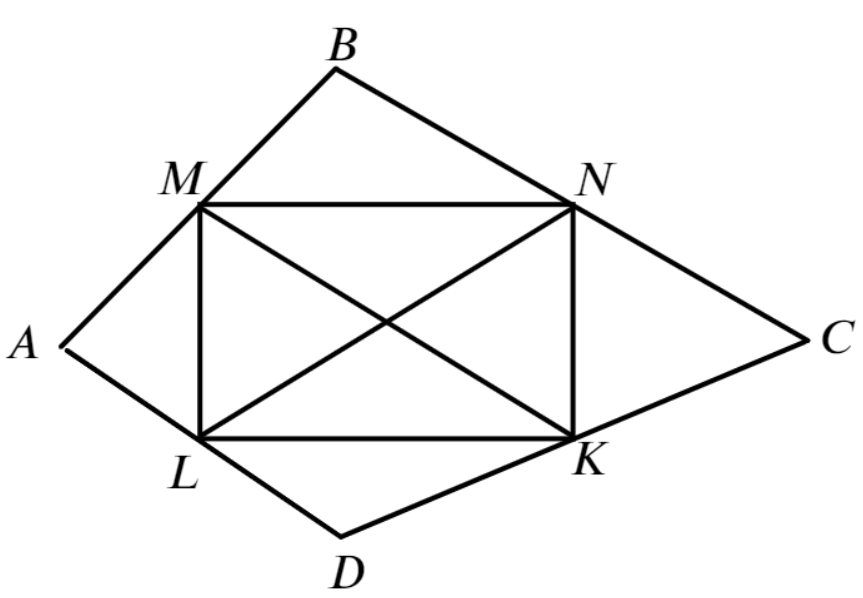
\includegraphics[scale=0.35]{g8-171.png}}
\end{figure}\\
Соединим все середины сторон. Тогда $MNKL$ --- это параллелограмм Вариньона (его противоположные стороны являются средними линиями, а значит параллельны диагоналям четырёхугольника и равны друг другу и половинам этих диагоналей). Так как по условию его диагонали равны, он является прямоугольником, стороны которого равны $6:2=3$ и $8:2=4.$ Тогда его по площадь равна $3\cdot4=12.$ Как известно (см., например, задачу 92), площадь исходного четырёхугольника в 2 раза больше, а значит она равна $12\cdot2=24.$\\
